\documentclass[11pt,a4paper]{article}
\usepackage[a4paper,margin=2.4cm]{geometry}
\usepackage{amsmath,amssymb,mathtools,amsthm}
\usepackage{fontspec}
\usepackage{polyglossia}
\setmainlanguage{english}
\setotherlanguage{russian}
\setmainfont{Liberation Serif}
\setsansfont{Liberation Sans}
\setmonofont{Liberation Mono}
\newfontfamily\cyrillicfont[Ligatures=TeX]{Liberation Serif}
\newfontfamily\cyrillicfontsf[Ligatures=TeX]{Liberation Sans}
\newfontfamily\cyrillicfonttt{Liberation Mono}
\usepackage{booktabs}
\usepackage{array}
\usepackage{enumitem}
\usepackage{graphicx}
\usepackage{float}
\usepackage{listings}
\usepackage{xcolor}
\usepackage[hidelinks]{hyperref}

\setlength{\parindent}{0pt}
\setlength{\parskip}{0.55em}
\emergencystretch=1.5em
\setlist{itemsep=0.25em,topsep=0.3em}
\lstset{basicstyle=\ttfamily\footnotesize,columns=fullflexible,keepspaces=true,
  frame=single,rulecolor=\color{black!25},breaklines=true,
  commentstyle=\color{black!55},showstringspaces=false}

\newcommand{\G}{\mathcal{G}_k}
\newcommand{\norm}[1]{\lVert #1\rVert_2}
\newcommand{\E}{\mathbb{E}}
\DeclareMathOperator*{\argmin}{arg\,min}
\DeclareMathOperator{\diag}{diag}
\DeclareMathOperator{\Var}{Var}

\title{Section 2: Implementation and numerical checks\\[0.2em]
\large illustrated on the noisy quadratic}
\author{Homework Mini-Project: SGD versus Robust SGD under Gradient Uncertainty}
\date{17 November 2026}

\begin{document}
\maketitle

\section*{Statement and summary}

Section 2 asks for four things: (i) a positive definite uncertainty matrix $S_k$
built from the per-example gradient observations by formula (4); (ii) a numerical
method for the robust subproblem (2), with its stopping criterion and cost;
(iii) an implementation of SGD and R-SGD and of the gradient observations for both
learning models (part (a)); (iv) numerical checks of the zero-radius limit, the
isotropic formula, the zero-step rule and the optimality condition of 1(d)
(part (b)), a study of the batch size (part (c)) and the documentation needed for
reproduction (part (d)). All checks are run on the noisy quadratic from the
Illustration; the gradient oracles of the two learning models are implemented and
verified as well, so that Section 3 can use the same code.

The main results:
\begin{itemize}
\item \textbf{Solver.} For diagonal $S_k$ problem (2) reduces exactly to one scalar
equation in $\tau=\sqrt{d^TS_kd}$, the \emph{secular equation}. It has a positive
root if and only if the zero-step condition (3) fails, so the solver reproduces
part 1(c) by construction. Newton's method on $\psi(\tau)=q(\tau)^{-1/2}-1$ is proved
to converge monotonically from $\tau_0=0$ (the function is concave), is exact in one
iteration for isotropic $S$, and needed on average 4.4 and at most 9 iterations on
20\,000 strongly anisotropic test problems. The cost is $O(p)$ per iteration.
\item \textbf{Checks.} The 1(d) optimality residual is at most $1.0\cdot10^{-14}$;
$\rho=0$ reproduces SGD bit for bit; the isotropic closed form is reproduced to
$4.8\cdot10^{-12}$; the zero-step rule agrees with (3) in $10\,000/10\,000$ cases,
including $\rho=(1\pm10^{-6})\rho_c$.
\item \textbf{Batch size.} $\widehat s_{k,j}$ is an unbiased estimate of
$\Var(g_{k,j})=\Sigma_{jj}/b$, its relative spread is $\sqrt{2/(b-1)}$ (141\% at
$b=2$, 9\% at $b=256$), and the statistic $g^TS^{-1}g$ grows linearly in $b$ away
from the minimiser. Consequently a fixed radius $\rho$ means less shrinkage and
fewer zero steps for larger batches; R-SGD tends to SGD as $b\to\infty$.
\end{itemize}

\begin{center}
\begin{tabular}{@{}llll@{}}
\toprule
Item of the task & What is shown & Where & Outcome \\
\midrule
$S_k$, formula (4) & unbiasedness, role of $\varepsilon_k$ & step 1 & proved, checked \\
solver for (2) & secular equation, Newton, cost & step 2 & proved, timed \\
(a) & SGD/R-SGD, gradient observations & step 3 & FD error $\le 5\cdot10^{-9}$ \\
(b) & four required tests & step 4 & all pass \\
(c) & batch size and $S_k$ & step 5 & theory = experiment \\
(d) & reproducibility & step 6 & seeds, settings, versions \\
\bottomrule
\end{tabular}
\end{center}

\section*{Setting and notation}

At iteration $k$ we have $b\ge2$ observations $v_{k,i}\in\mathbb R^p$ and
\begin{gather*}
g_k=\frac1b\sum_{i=1}^b v_{k,i},\qquad
\G=\{g_k+S_k^{1/2}u:\norm{u}\le\rho\},\\
d_k=\argmin_d\;\varphi_k(d),\qquad
\varphi_k(d)=g_k^Td+\rho\sqrt{d^TS_kd}+\frac{\norm{d}^2}{2\alpha_k}.
\end{gather*}
SGD uses $\theta_{k+1}=\theta_k-\alpha_kg_k$, R-SGD uses $\theta_{k+1}=\theta_k+d_k$.
Inside a single step I drop the index $k$: $g$, $S=\diag(s_1,\dots,s_p)$, $\alpha$.
The Mahalanobis norm of $g$ and the zero-step threshold are
\begin{equation*}
\kappa^2=g^TS^{-1}g=\sum_{j=1}^p\frac{g_j^2}{s_j},\qquad \rho_c=\kappa .
\end{equation*}

\textbf{Test problem (Illustration).}
$f(\theta)=\tfrac12(\theta_1^2+4\theta_2^2)$, $\nabla f(\theta)=(\theta_1,4\theta_2)^T$,
the Hessian is $\diag(1,4)$, hence $L=4$ and $\mu=1$; $\theta_0=(2,2)^T$,
$f(\theta_0)=10$, $f^\star=0$. The observations are
$v_{k,i}=\nabla f(\theta_k)+\sigma Az_{k,i}$, $A=\diag(2,\tfrac12)$,
$z_{k,i}\sim\mathcal N(0,I_2)$, so one observation has covariance
\begin{equation*}
\Sigma=\sigma^2AA^T=\sigma^2\diag\big(4,\tfrac14\big).
\end{equation*}
The noise is large along $\theta_1$, where the curvature is small, and small along
$\theta_2$, where the curvature is large: the signal-to-noise ratio is very different
in the two directions. Because $\Sigma$ is diagonal, the diagonal estimate (4) loses
nothing here; in the learning models it neglects the correlations between
parameters.

\section*{Step 1. The uncertainty matrix $S_k$ (formula (4))}

\begin{equation*}
\widehat s_{k,j}=\frac1{b(b-1)}\sum_{i=1}^b(v_{k,i,j}-g_{k,j})^2,\qquad
s_{k,j}=\widehat s_{k,j}+\varepsilon_k,\qquad
\varepsilon_k=10^{-3}\max\Big\{\frac1p\sum_j\widehat s_{k,j},\,10^{-8}\Big\}.
\end{equation*}

\subsection*{What $\widehat s_{k,j}$ estimates}

Let the observations be i.i.d.\ given $\theta_k$ with mean $m$ and covariance
$\Sigma$. Sampling \emph{with replacement} guarantees exactly this for the learning
models (step 5 shows what goes wrong without it). Then
$\Var(g_{k,j})=\Sigma_{jj}/b$. Using the identity
\begin{equation*}
\sum_{i=1}^b(v_{i,j}-g_j)^2=\sum_{i=1}^b(v_{i,j}-m_j)^2-b\,(g_j-m_j)^2
\end{equation*}
and taking expectations gives $\E\sum_i(v_{i,j}-g_j)^2=b\Sigma_{jj}-\Sigma_{jj}
=(b-1)\Sigma_{jj}$. Dividing by $b(b-1)$:
\begin{equation*}
\boxed{\;\E\,\widehat s_{k,j}=\frac{\Sigma_{jj}}b=\Var(g_{k,j})\;}
\end{equation*}
So $S_k$ is the (diagonal of the) covariance of the \emph{batch mean}, not of a single
observation. This is the right object: $\G$ describes the uncertainty of $g_k$.

\subsection*{Positive definiteness and the role of $\varepsilon_k$}

Every $s_{k,j}\ge\varepsilon_k\ge10^{-11}>0$, so $S_k\succ0$ always. The floor is
needed in two situations: a coordinate whose observations coincide (for example a
saturated $\tanh$ unit, or the bias of a model whose per-example gradients are equal),
and the noiseless quadratic ($\sigma=0$), where all $v_{k,i}$ coincide and
$\widehat s_k=0$. The relative part $10^{-3}\cdot\text{mean}(\widehat s)$ keeps the
floor scale-invariant: it bounds the ratio $\max_js_j/\min_js_j$ by about $10^3p$.
The absolute part $10^{-11}$ acts only when all $\widehat s_{k,j}$ vanish. Then
$S_k=\varepsilon_kI$, and by the isotropic formula of 1(d) R-SGD becomes
$d_k=-\alpha_k(1-\rho\sqrt{\varepsilon_k}/\norm{g_k})_+g_k$. This is SGD up to a
relative change $\rho\sqrt{\varepsilon_k}/\norm{g_k}$, except in the tiny region
$\norm{g_k}\le\rho\sqrt{\varepsilon_k}\approx3.2\cdot10^{-6}\rho$, which is checked
numerically in step 4.

\section*{Step 2. Solver for the robust subproblem (2)}

\subsection*{2.1 Trivial cases}
\begin{itemize}
\item $\rho=0$: $\varphi(d)=g^Td+\norm d^2/(2\alpha)$, so $d=-\alpha g$ (SGD), part 1(b).
\item $\kappa^2=g^TS^{-1}g\le\rho^2$: $d=0$, part 1(c). This test is exact and costs
$O(p)$. A step is counted as a \emph{zero step} only when this test fires, never by
comparing $\norm d$ with a tolerance. The case $g=0$ is included ($\kappa=0\le\rho$).
\end{itemize}

\subsection*{2.2 Reduction to one scalar equation}

Assume $\rho>0$ and $\kappa>\rho$. By part 1(c) the minimiser satisfies $d\neq0$, so
$\varphi$ is differentiable at $d$ and the condition of 1(d) holds:
\begin{equation*}
g+\rho\frac{Sd}{\sqrt{d^TSd}}+\frac d\alpha=0 .
\end{equation*}
Introduce the unknown scalar $\tau=\sqrt{d^TSd}>0$. Because $S$ is diagonal, the
vector equation splits into $p$ scalar equations,
$g_j+\rho s_jd_j/\tau+d_j/\alpha=0$, i.e.\
$d_j\big(\tfrac1\alpha+\tfrac{\rho s_j}{\tau}\big)=-g_j$. Multiplying by $\alpha\tau$:
\begin{equation*}
\boxed{\;d_j(\tau)=-\alpha\,\frac{\tau}{\tau+\alpha\rho s_j}\,g_j,\qquad j=1,\dots,p\;}
\end{equation*}
For every $\tau>0$ this $d(\tau)$ satisfies the optimality condition \emph{with
$\tau$ in place of $\sqrt{d^TSd}$}. It is the solution if and only if $\tau$ is
consistent with its definition, $\tau^2=\sum_js_jd_j(\tau)^2$. Substituting
$d_j(\tau)$ and dividing by $\tau^2>0$ gives the \emph{secular equation}
\begin{equation*}
q(\tau):=\sum_{j=1}^p\frac{a_j}{(\tau+c_j)^2}=1,\qquad
a_j=\alpha^2s_jg_j^2\ge0,\quad c_j=\alpha\rho s_j>0 .
\end{equation*}
(The name comes from the trust-region subproblem, where the same type of equation
appears; see Moré and Sorensen, 1983; Nocedal and Wright, 2006, §4.3.)

\subsection*{2.3 Existence and uniqueness of the root $\Longleftrightarrow$ (3) fails}

Since $g\ne0$, at least one $a_j>0$, and
\begin{equation*}
q'(\tau)=-2\sum_j\frac{a_j}{(\tau+c_j)^3}<0\quad(\tau\ge0),\qquad
q(0)=\sum_j\frac{\alpha^2s_jg_j^2}{\alpha^2\rho^2s_j^2}=\frac{\kappa^2}{\rho^2},\qquad
\lim_{\tau\to\infty}q(\tau)=0 .
\end{equation*}
$q$ is continuous and strictly decreasing, so $q(\tau)=1$ has a root in $(0,\infty)$
if and only if $q(0)>1$, i.e.\ $\kappa>\rho$, and then the root $\tau^\star$ is
unique. If $\kappa\le\rho$ there is no root, i.e.\ no nonzero point satisfies the
optimality condition, and the minimiser (which exists, $\varphi$ being strongly convex)
must be $d=0$. The solver therefore contains the zero-step rule 1(c) as the
non-existence case of its own equation. Because (2) is $1/\alpha$-strongly convex,
the stationary point $d(\tau^\star)$ is its unique global minimiser.

\textbf{Bracket.} Since $c_j>0$, $q(\tau)\le\sum_ja_j/\tau^2=\alpha^2g^TSg/\tau^2$.
Hence $q(\tau_{\rm hi})\le1$ for $\tau_{\rm hi}=\alpha\sqrt{g^TSg}$, and
$\tau^\star\in(0,\tau_{\rm hi}]$.

\subsection*{2.4 Newton's method on $\psi(\tau)=q(\tau)^{-1/2}-1$}

Instead of $q(\tau)-1$ (which is convex and behaves like $1/\tau^2$) I solve
$\psi(\tau)=q(\tau)^{-1/2}-1=0$. This function is increasing ($q$ decreases) and has
the following key property.

\textbf{Lemma (concavity).} $\psi$ is concave on $[0,\infty)$; it is affine if and
only if all $s_j$ with $g_j\ne0$ are equal.

\emph{Proof.} Write $x_j=1/(\tau+c_j)$ and $A_m=\sum_ja_jx_j^m$. Then
$q=A_2$, $q'=-2A_3$, $q''=6A_4$. For $F=q^{-1/2}$,
\begin{equation*}
F'=-\tfrac12q^{-3/2}q',\qquad
F''=q^{-5/2}\Big(\tfrac34q'^2-\tfrac12q\,q''\Big)=3\,q^{-5/2}\big(A_3^2-A_2A_4\big).
\end{equation*}
By the Cauchy--Schwarz inequality applied to the vectors $(\sqrt{a_j}\,x_j)_j$ and
$(\sqrt{a_j}\,x_j^2)_j$, $A_3^2\le A_2A_4$, so $F''\le0$. Equality holds if and only
if the two vectors are proportional, i.e.\ $x_j$ is the same for all $j$ with
$a_j>0$, i.e.\ all such $c_j=\alpha\rho s_j$ coincide. \hfill$\blacksquare$

\textbf{Monotone convergence from $\tau_0=0$.} We have $\psi(0)=\rho/\kappa-1<0$.
Newton's iteration is $\tau_{n+1}=\tau_n-\psi(\tau_n)/\psi'(\tau_n)$ with
$\psi'>0$. By concavity the tangent lies above the graph:
$\psi(\tau)\le\psi(\tau_n)+\psi'(\tau_n)(\tau-\tau_n)$. At $\tau=\tau_{n+1}$ the right
side is zero, so $\psi(\tau_{n+1})\le0$, i.e.\ $\tau_{n+1}\le\tau^\star$. Also
$\tau_{n+1}-\tau_n=-\psi(\tau_n)/\psi'(\tau_n)\ge0$. The iterates therefore increase
monotonically and stay below $\tau^\star$; the limit $\bar\tau$ satisfies
$\psi(\bar\tau)=0$ (continuity and $\psi'\ge\psi'(\tau^\star)>0$ on $[0,\tau^\star]$
by concavity), so $\bar\tau=\tau^\star$. Since $\psi$ is smooth with
$\psi'(\tau^\star)>0$, convergence is locally quadratic. In the isotropic case
$\psi$ is affine, and the first Newton step lands exactly on $\tau^\star$.

Why $q^{-1/2}$ and not $q-1$: in the isotropic case $q^{-1/2}=(\tau+c)/\sqrt{\sum a_j}$
is a straight line, and with anisotropy it stays close to one, so Newton needs very few
steps. For $q-1$, Newton from $\tau_0=0$ would also be monotone (convex decreasing
function), but much slower.

\textbf{Safeguard.} The iteration keeps the bracket $[\tau_{\rm lo},\tau_{\rm hi}]$
and replaces any Newton iterate outside it by bisection. By the argument above this
never happens in exact arithmetic; in 20\,000 test problems it was never triggered.

\subsection*{2.5 Stopping criterion and a-posteriori check}

The iteration stops when $|\psi(\tau_n)|\le10^{-14}$, or when the change
$|\tau_{n+1}-\tau_n|\le10^{-15}\tau_{n+1}$, or after 100 iterations (the maximum
observed was 9). Then $d=d(\tau_n)$ is returned.

What the criterion controls: $d(\tau)$ satisfies the optimality condition exactly
with $\tau$ in place of $\sqrt{d^TSd}$, and
$\sqrt{d(\tau)^TSd(\tau)}=\tau\sqrt{q(\tau)}=\tau/(1+\psi(\tau))$. Hence the only
error is the relative mismatch $|\psi|$ between $\tau$ and $\sqrt{d^TSd}$. After the
solve, the code also computes the residual of 1(d),
\begin{equation*}
r(d)=\frac{\norm{g+\rho Sd/\sqrt{d^TSd}+d/\alpha}}{\norm g},
\end{equation*}
and reports it (step 4).

\subsection*{2.6 Computational cost}

\begin{itemize}
\item Precomputing $a_j$, $c_j$, $\kappa^2$ costs $O(p)$; each Newton iteration
evaluates two sums, $O(p)$; memory is $O(p)$. Total: $O(p\cdot n_{\rm it})$ with
$n_{\rm it}\le9$ observed.
\item Building $g_k$ and $S_k$ from $V\in\mathbb R^{b\times p}$ costs $O(bp)$, and
computing $b$ per-example gradients costs $O(b\cdot\text{(one backprop)})$, which is
already $O(bp)$. Asymptotically the solver is therefore cheaper than the data it
consumes, by a factor of order $b/n_{\rm it}$.
\item \textbf{Measured wall-clock (Python/NumPy, one core).} Solver: 37\,µs at
$p=3$, 43\,µs at $p=33$, 82\,µs at $p=1000$, 4.7\,ms at $p=10^5$ (linear for large
$p$). For comparison, for the 33-parameter network with $b=32$: per-example gradients
18\,µs, $S_k$ 11\,µs. For models this small the solver time is dominated by Python
overhead and is \emph{not} negligible: one R-SGD update costs about 2--4 times an SGD
update in wall-clock, although both use exactly $b$ gradient evaluations. This must be
reported in Section 3 (runtime is a required output).
\item A general (non-diagonal) $S\succ0$ is handled by one eigendecomposition
$S=Q\Lambda Q^T$, $O(p^3)$: with $\tilde d=Q^Td$, $\tilde g=Q^Tg$ the problem becomes
$\tilde g^T\tilde d+\rho\sqrt{\tilde d^T\Lambda\tilde d}+\norm{\tilde d}^2/(2\alpha)$,
since $Q$ preserves the Euclidean norm, and the same diagonal solver applies.
\end{itemize}

\subsection*{2.7 What the formula says about the robust step}

The formula $d_j=-\alpha\,\frac{\tau^\star}{\tau^\star+\alpha\rho s_j}\,g_j$ shows
that R-SGD is SGD with a \emph{separate shrinkage factor in $(0,1)$ for every
coordinate}: the more uncertain a coordinate (larger $s_j$), the more it is shrunk.
Two limits are instructive.
\begin{itemize}
\item $\rho\to0$: $\tau^\star\to\alpha\sqrt{g^TSg}$, all factors tend to 1, $d\to-\alpha g$.
\item $\rho\uparrow\rho_c=\kappa$: $q(0)=\kappa^2/\rho^2\downarrow1$, so $\tau^\star\to0$.
Then $\tau^\star\ll\alpha\rho s_j$ and
$d_j\approx-\tau^\star g_j/(\rho s_j)$: the step vanishes \emph{continuously}, and its
\emph{direction} tends to $-S^{-1}g$, the gradient measured in units of its own
uncertainty.
\end{itemize}
Thus, for anisotropic $S$, increasing $\rho$ rotates the step from the SGD direction
$-g$ towards $-S^{-1}g$ while shortening it; for isotropic $S$ the direction stays
$-g$ and only the length changes. Figure~\ref{fig:sweep} shows both effects.

\section*{Step 3. Part (a): implementation of SGD and R-SGD}

\subsection*{3.1 One iteration}

Both methods are run by the same loop; the only difference is the step.
\begin{enumerate}
\item Obtain the observations $V\in\mathbb R^{b\times p}$, $V_{i\cdot}=v_{k,i}^T$ (3.2).
\item $g_k=$ mean of the rows of $V$; $\widehat s_k$, $\varepsilon_k$, $s_k$ by (4).
\item $\alpha_k=\alpha_0/\sqrt{1+k/50}$ (the same schedule for both methods).
\item SGD: $d_k=-\alpha_kg_k$. R-SGD: $d_k=$ \texttt{robust\_step}$(g_k,s_k,\alpha_k,\rho)$
(step 2), recording whether a zero step occurred, $\kappa_k^2$, the number of Newton
iterations and the residual $r(d_k)$.
\item $\theta_{k+1}=\theta_k+d_k$.
\end{enumerate}
SGD needs only $g_k$, but it receives the same $V$, so both methods use exactly $b$
gradient evaluations per update, i.e.\ $bK$ per run. The matrix $S_k$ is computed from
the \emph{same} observations $V$ that form $g_k$, as Section 3 requires (``construct
the uncertainty model from the gradient observations actually used in the update'').

\subsection*{3.2 Where the gradient observations come from}

All three oracles have the same interface \texttt{observe(theta, rng\_batch,
rng\_noise)} $\to V$.

\textbf{Noisy quadratic.} $V=\mathbf 1\,\nabla f(\theta_k)^T+\sigma ZA^T$, with
$Z\in\mathbb R^{b\times2}$ standard normal; there is no data set.

\textbf{Learning models.} Indices $i_1,\dots,i_b$ are drawn independently and
uniformly from $\{1,\dots,n\}$ \emph{with replacement}; the clean per-example
gradients $u_{i}(\theta_k)=\nabla_\theta\ell(t_\theta(a_{i}),y_{i})$ are computed in
closed form for the whole batch at once, and the corruption is added only to them:
$v_{k,i}=u_{i}(\theta_k)+\sigma z_{k,i}$, $z_{k,i}\sim\mathcal N(0,I_p)$. The training
data, the objective and every loss or accuracy evaluation stay clean.

\emph{Why per-example gradients, and not the gradient of the batch loss:} $S_k$ is
built from the spread of the individual $v_{k,i}$ around $g_k$, so the $b$ vectors are
needed separately. With an automatic-differentiation framework one would use, e.g.,
\texttt{torch.func.vmap(grad(...))}; here the closed forms below are cheaper and exact.

\textbf{Logistic regression} ($t=w^Ta+c$, $\theta=(w_1,w_2,c)$, $p=3$). With
$\ell(t,y)=\log(1+e^t)-yt$,
\begin{equation*}
\frac{\partial\ell}{\partial t}=\frac{e^t}{1+e^t}-y=\operatorname{sigm}(t)-y,\qquad
\nabla_\theta t=(a^T,1)^T\quad\Longrightarrow\quad
u_i(\theta)=\big(\operatorname{sigm}(t_i)-y_i\big)\begin{pmatrix}a_i\\1\end{pmatrix}.
\end{equation*}
The loss is evaluated stably as \texttt{logaddexp(0,t) - y*t}, the sigmoid as
\texttt{scipy.special.expit}.

\textbf{Two-layer network} ($t=w_2^T\tanh(W_1a+b_1)+b_2$, $p=16+8+8+1=33$, parameter
order $(\mathrm{vec}_{\rm row}W_1,b_1,w_2,b_2)$). With $z=W_1a+b_1$, $h=\tanh z$,
$\delta=\operatorname{sigm}(t)-y$, back-propagation gives
\begin{equation*}
\frac{\partial\ell}{\partial b_2}=\delta,\quad
\frac{\partial\ell}{\partial w_2}=\delta\,h,\quad
\frac{\partial\ell}{\partial b_1}=\delta\,w_2\odot(1-h\odot h)=:e,\quad
\frac{\partial\ell}{\partial W_1}=e\,a^T,
\end{equation*}
evaluated for all $b$ examples by broadcasting (a $b\times33$ matrix). Documented
initialisation (for Section 3): $W_1\sim\mathcal N(0,\tfrac12)$, $b_1=0$,
$w_2\sim\mathcal N(0,\tfrac18)$, $b_2=0$ (variance $1/\text{fan-in}$).

\textbf{Verification by finite differences.} For 5 random parameter vectors per model
(200 points of each data set), central differences with $h=10^{-6}$ were compared
with (i) the mean of the per-example gradients versus the gradient of the mean loss
and (ii) each of 20 per-example gradients versus the single-example loss:

\begin{center}
\begin{tabular}{@{}lcc@{}}
\toprule
Model & max rel.\ error, mean gradient & max rel.\ error, per example \\
\midrule
logistic regression ($p=3$) & $3.2\cdot10^{-10}$ & $4.6\cdot10^{-9}$ \\
two-layer network ($p=33$) & $6.3\cdot10^{-10}$ & $5.3\cdot10^{-10}$ \\
\bottomrule
\end{tabular}
\end{center}
These errors are at the level of the finite-difference truncation and rounding errors
($\approx h^2$ and $\approx\epsilon_{\rm mach}/h$), so the analytic gradients are correct.

\section*{Step 4. Part (b): numerical checks}

Random test problems for the solver are deliberately hard: $g\sim\mathcal N(0,I_p)$,
$s_j$ log-uniform over six decades $[10^{-3},10^3]$, $\alpha$ log-uniform in
$[10^{-2},1]$, $p\in\{2,3,33,1000\}$, and $\rho=m\rho_c$ with $m$ chosen as stated
below. Every number in this report is produced by \texttt{checks\_section2.py} and
stored in \texttt{results\_section2.json}.

\subsection*{4.1 Zero-radius limit}
\begin{itemize}
\item $\rho=0$ exactly: $d=-\alpha g$ bit for bit in $1000/1000$ random problems
($p$ from 1 to 49).
\item $\rho\to0^+$: for five problems with $p=33$ and
$\rho=10^{-1},\dots,10^{-8}$ the deviation $\norm{d(\rho)+\alpha g}/(\alpha\norm g)$
decreases linearly in $\rho$; the fitted log--log slopes are $0.995$--$0.999$, and at
$\rho=10^{-8}$ the deviation is at most $1.5\cdot10^{-8}$. The robust step is
therefore continuous at $\rho=0$, with a first-order change.
\item Trajectories: SGD and R-SGD with $\rho=0$, run on the quadratic ($\sigma=1$,
$b=8$, 300 updates) with the same seeds, coincide exactly (maximum difference 0).
\end{itemize}

\subsection*{4.2 Isotropic formula}

$10\,000$ problems with $S=sI$: $p\in\{1,\dots,50\}$, $s$ log-uniform in
$[10^{-4},10^2]$, and $\rho$ set so that the ratio $\rho\sqrt s/\norm g$ is uniform on
$[0,2]$, which covers both branches of $(\cdot)_+$ equally. The solver was compared with
\begin{equation*}
d=-\alpha\Big(1-\frac{\rho\sqrt s}{\norm g}\Big)_+g .
\end{equation*}
\begin{itemize}
\item branch (zero or nonzero) agrees in $10\,000/10\,000$ cases (4949 zero steps);
\item for the 5051 nonzero steps the maximum relative error is $4.8\cdot10^{-12}$;
\item every nonzero step took exactly \textbf{one} Newton iteration, as the lemma of
2.4 predicts ($\psi$ is affine);
\item $g=0$ gives $d=0$ through the zero-step test, as required in 1(d).
\end{itemize}

\subsection*{4.3 Zero-step rule}

For each $m\in\{0.5,0.9,0.99,0.999,1-10^{-6},1+10^{-6},1.001,1.01,1.1,2\}$, 1000
anisotropic problems with $\rho=m\rho_c$ were solved. The solver returned exactly
$d=0$ if and only if $m>1$, in $1000/1000$ cases for every $m$, including
$m=1\pm10^{-6}$. Figure~\ref{fig:sweep}(a) shows how $\norm d$ goes to zero
continuously as $\rho\uparrow\rho_c$ and stays zero beyond; panel (b) shows the
rotation of the direction from $-g$ to $-S^{-1}g$ predicted in 2.7 (for this example the
angle between $g$ and $S^{-1}g$ is $57.8^\circ$).

\begin{figure}[H]
\centering
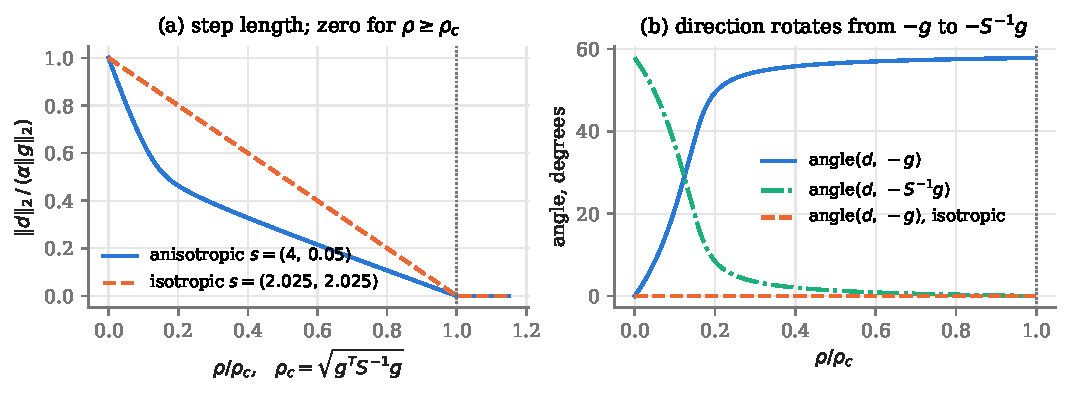
\includegraphics[width=\linewidth]{../fig/zero_step_sweep.pdf}
\caption{Robust step for $g=(1,\,0.6)$, $\alpha=0.5$ as a function of $\rho/\rho_c$.
Anisotropic $s=(4,\,0.05)$, $\rho_c=2.73$; isotropic $s$ with the same mean,
$\rho_c=0.82$. (a) Step length relative to SGD; it reaches zero exactly at
$\rho=\rho_c$. (b) Angle of $d$ to $-g$ and to $-S^{-1}g$; for isotropic $S$ the direction
never changes.}
\label{fig:sweep}
\end{figure}

\subsection*{4.4 Optimality condition of 1(d) and independent cross-checks}

\begin{center}
\begin{tabular}{@{}p{0.47\linewidth}p{0.45\linewidth}@{}}
\toprule
Check & Result \\
\midrule
Residual $r(d)$ of 1(d), 20\,000 random problems, $m\sim U(0.001,0.999)$ &
$\max r=1.0\cdot10^{-14}$ \\
Residual along all R-SGD trajectories of 4.5 & $\max r=9.9\cdot10^{-15}$ \\
Newton iterations, 20\,000 problems &
mean 4.4, median 4, 99\% quantile 7, max 9 \\
Safeguard bisections / non-monotone Newton iterates & $0$ / $0$ (5000 unsafeguarded runs) \\
Saddle point of (1): $d=-\alpha h^\star$,
$h^\star=g+\rho Sd/\sqrt{d^TSd}$ (part 1(a)) &
$\max\norm{d+\alpha h^\star}/\norm d=6.0\cdot10^{-12}$ \\
CVXPY (Clarabel), SOCP form, 300 problems ($s_j$ over four decades, $m\sim U(0.05,0.95)$) &
our objective never larger: $\max(\varphi_{\rm ours}-\varphi_{\rm cvx})/|\varphi|=1.8\cdot10^{-15}$ \\
& $\norm{d-d_{\rm cvx}}/\norm d$: median $4.0\cdot10^{-7}$, max $4.0\cdot10^{-4}$ \\
Strong-convexity certificate,
$\varphi(d+\delta)-\varphi(d)\ge\norm\delta^2/(2\alpha)$,
15\,000 random $\delta$ &
smallest relative slack $-1.6\cdot10^{-15}$ (rounding only) \\
\bottomrule
\end{tabular}
\end{center}

Remarks.
\begin{itemize}
\item The SOCP form used for CVXPY is
$\min_{d,t}\;g^Td+\rho t+\norm d^2/(2\alpha)$ s.t.\ $\norm{S^{1/2}d}\le t$. Its
solutions differ from ours by up to $4\cdot10^{-4}$ because an interior-point method
reaches only about $10^{-8}$ in the objective (Clarabel flagged 135 of 300 solves as
``optimal\_inaccurate'' at the requested tolerance $10^{-12}$). Since $\varphi$ is
$1/\alpha$-strongly convex, $\norm{d_{\rm cvx}-d^\star}^2\le2\alpha(\varphi(d_{\rm cvx})-\varphi(d^\star))$,
so an objective gap of $10^{-8}$ explains a distance of $10^{-4}$. Our objective was
never larger than CVXPY's.
\item The certificate test is a direct proof of optimality: for the exact minimiser of
a $1/\alpha$-strongly convex function the inequality holds for every $\delta$, and it
fails for small $\delta$ along a descent direction at any non-optimal point.
\item The saddle-point error is the residual measured differently:
$d+\alpha h^\star=\alpha\,(g+\rho Sd/\tau+d/\alpha)$, so it is amplified by
$\alpha\norm g/\norm d$, which is large just below the threshold.
\end{itemize}

\subsection*{4.5 Zero steps along trajectories of the noisy quadratic}

This is an illustration, not a tuned comparison: $b=8$, $\alpha_0=0.2$ (below
$2/L=0.5$), $\alpha_k=\alpha_0/\sqrt{1+k/50}$, $K=300$ updates, $\theta_0=(2,2)$, 20
seeds with common random numbers (both methods see the same $z_{k,i}$), and
$\rho\in\{1,\,2.45\}$. The value $2.45\approx\sqrt{\chi^2_{2,0.95}}$ is the radius at
which, for large $b$, 95\% of updates at the minimiser are zero steps (step 5).

\begin{center}
\begin{tabular}{@{}llcccc@{}}
\toprule
$\sigma$ & method & median final $f$ [IQR] & zero steps & max $f$ at a zero step & mean Newton it. \\
\midrule
0 & SGD & $6.3\cdot10^{-31}$ & -- & -- & -- \\
0 & R-SGD $\rho=1$ & $5.0\cdot10^{-12}$ & 0 & -- & 1.0 \\
0 & R-SGD $\rho=2.45$ & $3.0\cdot10^{-11}$ & 0 & -- & 1.0 \\
\midrule
1 & SGD & $0.0034$ [0.0020, 0.0067] & -- & -- & -- \\
1 & R-SGD $\rho=1$ & $0.0016$ [0.0005, 0.0073] & 33.0\% & 0.94 & 4.3 \\
1 & R-SGD $\rho=2.45$ & $0.0196$ [0.0085, 0.0386] & 80.8\% & 1.59 & 4.1 \\
\midrule
4 & SGD & $0.054$ [0.033, 0.107] & -- & -- & -- \\
4 & R-SGD $\rho=1$ & $0.026$ [0.008, 0.116] & 33.7\% & 2.50 & 4.3 \\
4 & R-SGD $\rho=2.45$ & $0.126$ [0.027, 0.269] & 85.0\% & 2.94 & 3.9 \\
\bottomrule
\end{tabular}
\end{center}

\begin{figure}[H]
\centering
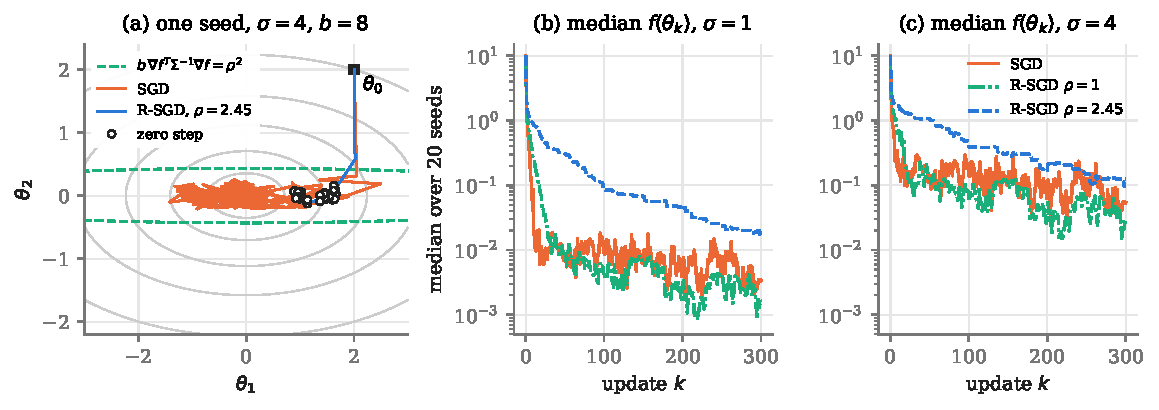
\includegraphics[width=\linewidth]{../fig/quadratic_trajectories.pdf}
\caption{Noisy quadratic, $b=8$, $\alpha_0=0.2$, 300 updates. (a) One seed at
$\sigma=4$: SGD and R-SGD ($\rho=2.45$) with identical noise draws; circles mark the
points where R-SGD took a zero step; the dashed ellipse is
$b\,\nabla f^T\Sigma^{-1}\nabla f=\rho^2$ (semi-axes $6.9$ and $0.43$, so in this window
it appears as a horizontal strip). (b), (c) Median of $f(\theta_k)$ over 20 seeds.}
\label{fig:traj}
\end{figure}

What these numbers show:
\begin{itemize}
\item \textbf{Zero steps happen far from the minimiser.} At $\sigma=4$, $\rho=2.45$,
zero steps occurred at points with $f$ up to $2.94$ (with $f(\theta_0)=10$ and
$f^\star=0$), where $\norm{\nabla f}$ is far from zero. Figure~\ref{fig:traj}(a) shows
why: along $\theta_1$ the gradient $\theta_1$ is weak and the noise (standard deviation
$2\sigma$ per observation) is strong, so the expected statistic
$b\,\nabla f^T\Sigma^{-1}\nabla f=b\big(\theta_1^2/(4\sigma^2)+64\theta_2^2/\sigma^2\big)$
stays below $\rho^2$ for $|\theta_1|$ up to $\rho\cdot2\sigma/\sqrt b=6.9$. R-SGD quickly
fixes $\theta_2$, whose signal-to-noise ratio is high, and then stalls in $\theta_1$.
This is the numerical counterpart of the answer to 1(c): (3) does not imply
$\nabla f(\theta_k)=0$.
\item \textbf{The $\varepsilon_k$ floor at $\sigma=0$.} All observations coincide,
$S_k=10^{-11}I$, and R-SGD converges to the boundary of its zero-step region,
$\norm{\nabla f}=\rho\sqrt{\varepsilon}$, where $f\approx\norm{\nabla f}^2/2=\rho^2\varepsilon/2$:
$5.0000\cdot10^{-12}$ for $\rho=1$ and $3.0013\cdot10^{-11}$ for $\rho=2.45$, matching
the measured medians to nine digits. The approach is continuous, which is why no exact
zero step was recorded. Since $S=\varepsilon I$ is isotropic, Newton took one iteration
at every update.
\item \textbf{A moderate radius can help; a large radius stalls.} $\rho=1$ lowered the
median final $f$ (0.0016 vs 0.0034 at $\sigma=1$; 0.026 vs 0.054 at $\sigma=4$), but the
interquartile ranges overlap, and $\rho=2.45$ was worse than SGD at both noise levels.
These are untuned illustration runs; whether the gain survives a fair tuning of
$\alpha_0$ for both methods, and whether it is more than a shorter step, is a
question for Sections 4--5.
\item \textbf{Cost.} Both methods used $2400=bK$ gradient evaluations per run; the
wall-clock was about 4--7\,ms per run for SGD and 9--23\,ms for R-SGD (runs with many
zero steps are faster, since a zero step skips Newton).
\end{itemize}

\section*{Step 5. Part (c): how the batch size affects the uncertainty estimate}

\subsection*{5.1 Theory}

Fix $\theta$ and let the observations be Gaussian, as in the quadratic:
$v_{i,j}\sim\mathcal N(\mu_j,\Sigma_{jj})$ i.i.d., with independent coordinates
($A$ diagonal). Standard facts about Gaussian samples give:
\begin{enumerate}
\item \textbf{Mean.} $\E\widehat s_j=\Sigma_{jj}/b$ (step 1): the estimate itself
shrinks like $1/b$, because it estimates the variance of the mean.
\item \textbf{Spread.} $(b-1)\,b\,\widehat s_j/\Sigma_{jj}\sim\chi^2_{b-1}$, hence
$\operatorname{sd}(\widehat s_j)/\E\widehat s_j=\sqrt{2/(b-1)}$: 141\% at $b=2$, 53\% at
$b=8$, 9\% at $b=256$. With a small batch $S_k$ is itself very noisy.
\item \textbf{Zero-step statistic.} $g_j$ and $\widehat s_j$ are independent, and
$\E[1/\chi^2_\nu]=1/(\nu-2)$, so (neglecting $\varepsilon_k$)
\begin{align*}
\E\big[g^TS^{-1}g\big]&=\sum_j\E[g_j^2]\,\E[1/\widehat s_j]
=\sum_j\Big(\mu_j^2+\frac{\Sigma_{jj}}b\Big)\frac{b}{\Sigma_{jj}}\,\frac{b-1}{b-3}\\
&=\big(b\,\mu^T\Sigma^{-1}\mu+p\big)\frac{b-1}{b-3},\qquad b>3 .
\end{align*}
Away from a stationary point ($\mu\ne0$) the statistic grows \emph{linearly} in $b$, so
for fixed $\rho$ zero steps disappear as $b$ grows. At a stationary point ($\mu=0$)
each $g_j/\sqrt{\widehat s_j}$ is Student-$t$ with $b-1$ degrees of freedom, the mean is
$p(b-1)/(b-3)$, and for $b\le3$ it is infinite (heavy tails). For large $b$,
$g^TS^{-1}g\to\chi^2_p$ in distribution, which gives a natural scale for $\rho$:
$\rho=\sqrt{\chi^2_{p,0.95}}$ ($=2.45$ for $p=2$) means 95\% zero steps at the minimiser.
\item \textbf{Size of the robust correction.} The uncertainty radius in gradient
units is $\rho\sqrt{s_j}\propto\rho/\sqrt b$, so the shrinkage factors of 2.7 tend to 1
and R-SGD tends to SGD as $b\to\infty$ with $\rho$ fixed. In other words $\rho$ and $b$
are not independent knobs: the same $\rho$ means a different amount of robustness at
different batch sizes.
\end{enumerate}

\subsection*{5.2 Numerical check}

$\sigma=1$ (so $\Sigma=\diag(4,\tfrac14)$), $20\,000$ independent batches for each $b$,
at three fixed points: the minimiser $\theta^\star=(0,0)$, an intermediate point
$\theta_{\rm mid}=(1,\,0.1)$ with $\mu^T\Sigma^{-1}\mu=0.89$, and $\theta_0=(2,2)$ with
$\mu^T\Sigma^{-1}\mu=257$. Zero steps are counted for $\rho=2.45$; the last column is
the mean relative change of the step,
$\norm{d+\alpha g}/(\alpha\norm g)$, at $\theta_{\rm mid}$ for $\rho=1$, $\alpha=0.1$.

\begin{center}
\small
\setlength{\tabcolsep}{4.2pt}
\begin{tabular}{@{}rccccccccc@{}}
\toprule
& \multicolumn{2}{c}{$b\,\E\widehat s_j/\Sigma_{jj}$} & \multicolumn{2}{c}{rel.\ sd of $\widehat s_1$}
& \multicolumn{2}{c}{$\E\,g^TS^{-1}g$ at $\theta^\star$} & \multicolumn{2}{c}{zero-step freq.} & rel.\ change \\
\cmidrule(lr){2-3}\cmidrule(lr){4-5}\cmidrule(lr){6-7}\cmidrule(lr){8-9}
$b$ & $j=1$ & $j=2$ & emp. & $\sqrt{2/(b-1)}$ & emp. & theory & $\theta^\star$ & $\theta_{\rm mid}$ & at $\theta_{\rm mid}$ \\
\midrule
2 & 1.002 & 1.013 & 1.415 & 1.414 & 788.47 & $\infty$ & 0.558 & 0.410 & 0.579 \\
3 & 0.998 & 1.011 & 1.011 & 1.000 & 13.27 & $\infty$ & 0.719 & 0.484 & 0.606 \\
4 & 1.003 & 1.000 & 0.819 & 0.816 & 5.32 & 6.00 & 0.794 & 0.479 & 0.604 \\
8 & 0.994 & 0.999 & 0.534 & 0.535 & 2.78 & 2.80 & 0.885 & 0.297 & 0.536 \\
16 & 0.999 & 1.003 & 0.365 & 0.365 & 2.30 & 2.31 & 0.922 & 0.076 & 0.441 \\
32 & 0.998 & 1.003 & 0.251 & 0.254 & 2.14 & 2.14 & 0.938 & 0.001 & 0.338 \\
64 & 1.001 & 0.998 & 0.178 & 0.178 & 2.04 & 2.07 & 0.946 & 0.000 & 0.237 \\
128 & 0.999 & 1.000 & 0.126 & 0.125 & 2.02 & 2.03 & 0.946 & 0.000 & 0.167 \\
256 & 1.001 & 1.000 & 0.089 & 0.089 & 1.99 & 2.02 & 0.952 & 0.000 & 0.117 \\
\bottomrule
\end{tabular}
\end{center}
At $\theta_0$ the zero-step frequency was $0$ for every $b$.

\begin{figure}[H]
\centering
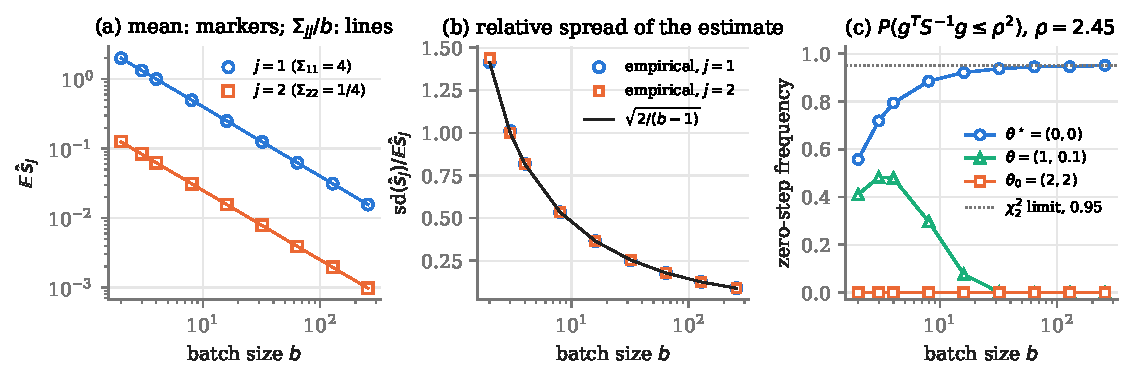
\includegraphics[width=\linewidth]{../fig/batch_size.pdf}
\caption{Batch size and the uncertainty estimate (noisy quadratic, $\sigma=1$,
$20\,000$ batches per $b$). (a) $\E\widehat s_j$ follows $\Sigma_{jj}/b$. (b) The
relative spread follows $\sqrt{2/(b-1)}$. (c) Zero-step frequency for $\rho=2.45$ at
three points; at $\theta^\star$ it tends to the $\chi^2_2$ value $0.95$.}
\label{fig:batch}
\end{figure}

Reading of the results:
\begin{itemize}
\item Points 1 and 2 of 5.1 are confirmed to within Monte Carlo error at every $b$
(ratios $1.00\pm0.013$; spreads within $0.025$ of $\sqrt{2/(b-1)}$).
\item The mean of $g^TS^{-1}g$ at $\theta^\star$ matches $p(b-1)/(b-3)$ for $b\ge8$. For
$b=2,3$ the theoretical mean is infinite and the sample means (788 and 13) are
meaningless; at $b=4$ the variance of the statistic is infinite, so the sample mean
converges slowly (5.3 vs 6.0). This is the heavy-tail effect of a two- or
three-point variance estimate.
\item At $\theta_{\rm mid}$ the zero-step frequency falls from about $0.4$--$0.5$ to
$0$ between $b=4$ and $b=32$: the transition happens where
$b\,\mu^T\Sigma^{-1}\mu\approx\rho^2$, i.e.\ $b\approx6/0.89\approx7$. The frequency is
\emph{not} monotone for $b\le4$: with very small batches $\widehat s_j$ is often tiny by
chance, $g^TS^{-1}g$ explodes and the zero step is avoided. Zero-step decisions at
$b\le4$ are therefore largely random.
\item The robust correction shrinks like $1/\sqrt b$: from $b=64$ to $b=256$ the
relative change halves ($0.237\to0.117$). With a fixed $\rho$, R-SGD at large $b$ is
nearly SGD.
\end{itemize}

\subsection*{5.3 Why sampling with replacement}

For the learning models the observations come from a finite training set of size $n$.
With replacement the $b$ draws are i.i.d.\ and $\E\widehat s_j=\Var(g_j)$ exactly.
Without replacement the variance of the batch mean has the finite-population factor
$(n-b)/(n-1)$, while the sample variance still estimates the population variance, so
$\widehat s_j$ overestimates $\Var(g_j)$ by the factor $n/(n-b)$. Check on a logistic
regression data set with $n=64$, $\sigma=0$, $20\,000$ batches:

\begin{center}
\begin{tabular}{@{}ccccc@{}}
\toprule
$n$ & $b$ & $\E\widehat s_j/\Var(g_j)$, with repl. & without repl. & predicted $n/(n-b)$ \\
\midrule
64 & 8 & 1.000--1.002 & 1.139--1.143 & 1.143 \\
64 & 32 & 0.999--1.003 & 2.000--2.004 & 2.000 \\
\bottomrule
\end{tabular}
\end{center}
(Ranges are over the three coordinates $w_1,w_2,c$.) Without replacement and with
$b=n/2$ the uncertainty would be overstated by a factor of 2, which would produce
spurious zero steps.

\section*{Step 6. Part (d): what is needed to reproduce the results}

\begin{itemize}
\item \textbf{Code.} \texttt{rsgd.py} (estimator (4), solver, SGD/R-SGD loop, oracles,
data generators, finite-difference check) and \texttt{checks\_section2.py} (every
number, table and figure of this report). Run: \texttt{python checks\_section2.py};
the full run takes about 20\,s.
\item \textbf{Random numbers.} One master seed $20261117$; the experiments use
independent child streams from \texttt{numpy.random.SeedSequence(20261117).spawn(8)}.
Inside an optimisation run there are two separate generators, one for batch indices
and one for gradient noise $z_{k,i}$ (in Section 3 also one for data and one for
initialisation).
\item \textbf{Common random numbers.} SGD and R-SGD are started from fresh generators
with the same seeds, so in a paired comparison they receive the same batch indices and
the same draws $z_{k,i}$ at every iteration (the observations still differ once the
iterates differ, since $u_i$ is evaluated at different $\theta_k$).
\item \textbf{Corruption model.} The noise is added only to the observations $V$.
The objective $f$, the training data, and all losses and accuracies are evaluated on
clean data.
\item \textbf{Settings.} float64 throughout; $b$, $\alpha_0$, schedule
$\alpha_0/\sqrt{1+k/50}$, number of updates $K$, $\rho$, $\sigma$, $\theta_0$ as stated in
each check; $\varepsilon_k$ exactly as in (4); solver tolerances
$|\psi|\le10^{-14}$, relative step $\le10^{-15}$, at most 100 iterations; a zero step is
recorded only when $g^TS^{-1}g\le\rho^2$.
\item \textbf{Reported per run.} Gradient evaluations ($bK$ for both methods),
wall-clock time, zero-step count, Newton iterations, maximum residual of 1(d).
\item \textbf{Software.} Python 3.13.18, NumPy 2.5.3, SciPy 1.18.1, Matplotlib 3.11.2,
CVXPY 1.9.3 (Clarabel) only for the cross-check.
\end{itemize}

\section*{Conclusions for the next sections}

\begin{itemize}
\item The solver is exact up to rounding, robust and cheap in flops; in pure Python its
fixed overhead makes R-SGD 2--4 times slower per update than SGD for models of 3 and 33
parameters, so runtime must be reported next to gradient-evaluation counts.
\item Zero steps are a statement about the signal-to-noise ratio of the mini-batch
gradient, not about stationarity. They appear far from the minimiser when the noise is
strong in a low-curvature direction.
\item $\rho$, $b$ and the noise level interact: the zero-step region scales like
$\rho\sigma/\sqrt b$, and the robust correction like $\rho/\sqrt b$. A fair comparison in
Section 4 must tune $\rho$ at the batch size actually used. Because the correction is
largely a shortening of the step, it must be compared with SGD at a smaller $\alpha_0$.
\item With $b\le4$ the estimate $S_k$ is too noisy (relative spread $\ge 82\%$) for
reliable zero-step decisions; $b\ge8$ is advisable.
\end{itemize}

\textbf{References.}
J.~J.~Moré, D.~C.~Sorensen, Computing a trust region step, \emph{SIAM J.\ Sci.\
Stat.\ Comput.} 4 (1983) 553--572.
J.~Nocedal, S.~J.~Wright, \emph{Numerical Optimization}, 2nd ed., Springer, 2006, §4.3.

\section*{Appendix: the solver}

\begin{lstlisting}[language=Python]
def robust_step(g, s, alpha, rho, tol=1e-14, maxit=100):
    kappa2 = np.sum(g * g / s)                    # g^T S^{-1} g
    if rho == 0.0:                                # SGD
        return -alpha * g
    if kappa2 <= rho * rho:                       # zero-step rule (3)
        return np.zeros_like(g)
    a = alpha**2 * s * g * g                      # q(tau) = sum a/(tau+c)^2
    c = alpha * rho * s
    def psi_and_deriv(tau):
        den = tau + c
        q, dq = np.sum(a / den**2), -2.0 * np.sum(a / den**3)
        return q**-0.5 - 1.0, -0.5 * q**-1.5 * dq
    lo, hi = 0.0, alpha * np.sqrt(np.sum(s * g * g))   # bracket
    tau = 0.0
    psi, dpsi = psi_and_deriv(tau)
    for it in range(maxit):
        tau_new = tau - psi / dpsi                # Newton (monotone from 0)
        if not (lo < tau_new <= hi):
            tau_new = 0.5 * (lo + hi)             # safeguard, never used
        step, tau = abs(tau_new - tau), tau_new
        psi, dpsi = psi_and_deriv(tau)
        lo, hi = (tau, hi) if psi < 0 else (lo, tau)
        if abs(psi) <= tol or step <= 1e-15 * tau:
            break
    return -alpha * tau * g / (tau + c)
\end{lstlisting}

\end{document}
